\section{Accelerated Sampling Methods}
\label{section:accel}

\subsection{Accelerated Molecular Dynamics}
\label{section:accelmd}
Accelerated molecular dynamics (aMD)~\cite{HAME2004mc} is an enhanced-sampling method that
improves the conformational space sampling by 
reducing energy barriers separating different states of a system.
The method modifies the potential 
energy landscape by raising energy wells that are below
a certain threshold level, while leaving those above this level unaffected.
As a result, barriers separating adjacent energy basins are reduced, allowing the system to sample
conformational space that cannot be easily accessed in a classical MD simulation.

Please include the following two references in your work using the NAMD implementation of aMD:
\begin{itemize}
  \item {Accelerated Molecular Dynamics: A Promising and Efficient Simulation Method for Biomolecules, D.\,Hamelberg, J.\,Mongan, and J.\,A. McCammon. {\it J. Chem. Phys.}, 120:11919-11929, 2004.}
  \item{Implementation of Accelerated Molecular Dynamics in NAMD, Y.\,Wang, C.\,Harrison, K.\,Schulten, and J.\,A. McCammon, {\it Comp.~Sci.~Discov.}, 4:015002, 2011.}
\end{itemize}

\subsubsection{Theoretical background}
In the original form of aMD~\cite{HAME2004mc}, when the system's potential energy falls       
below a threshold energy, $E$, a boost potential is added, 
such that the modified potential, $V^*({\bf r})$, is related to the original
potential, $V({\bf r})$, via
\begin{equation}
V^*({\bf r})= V({\bf r}) + \Delta V({\bf r}),
\end{equation}
where $\Delta V({\bf r})$ is the boost potential, 
\begin{equation} 
\Delta V({\bf r})= \left \{
\begin{array}{l l}
0   & \quad \quad V({\bf r})\geq E \\  
\frac{(E-V({\bf r}))^2}{\alpha+E-V({\bf r})}  & \quad \quad V({\bf r})<E. \\
\end{array} \right. 
\end{equation}
As shown in the following figure, the threshold energy $E$ controls the portion of 
the potential surface affected by the boost, while the acceleration factor 
$\alpha$ determines the shape of the modified potential.
%as $\alpha$ increases, the modified potential asymptotically approaches the original potential;
%as $\alpha$ decreases, the energy surface below $E$ begins to resemble a constant potential.
Note that $\alpha$ cannot be set to zero, otherwise the derivative of the modified potential
is discontinuous.

\begin{figure}[!ht]
  \centering
  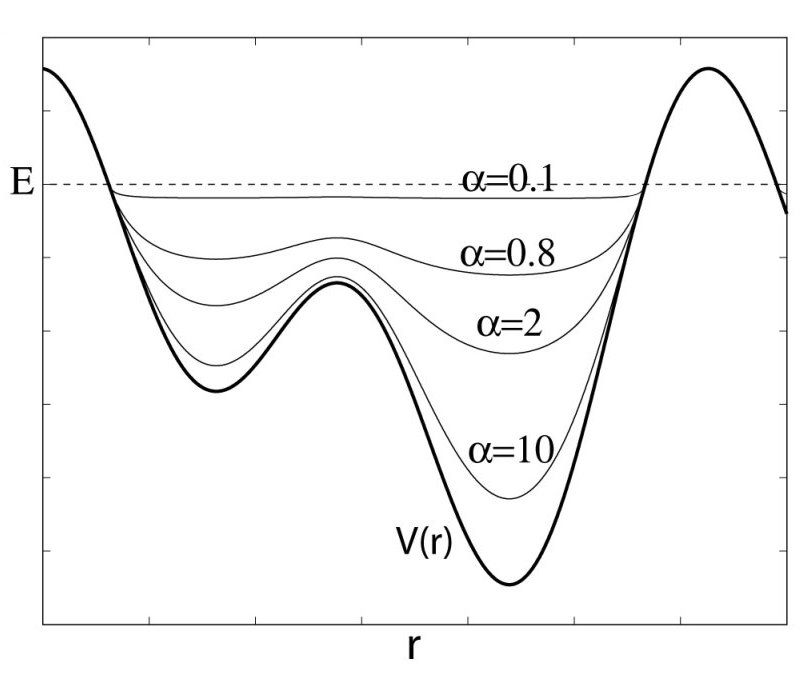
\includegraphics[width=7cm]{figures/amd_schematic.jpg}
  \caption{Schematics of the aMD method. When the original potential (thick line) falls below a threshold energy $E$ (dashed line),
          a boost potential is added. The modified energy profiles (thin lines) have smaller barriers separating adjacent
	  energy basins. 
	  %Two parameters, $E$ and $\alpha$, controls the portion of the affected potential landscape and the
	  %shape of the modified potential, respectively.
	  }
  \label{fig:amd_schematic}
\end{figure}
From an aMD simulation, the ensemble average, $\langle A \rangle$, of an observable, $A({\bf r})$, can be calculated
using the following reweighting procedure:
\begin{equation}
\langle A \rangle =\frac{\langle A({\bf r})\,\text{exp} (\beta \Delta V({\bf r})) \rangle^* }
{\langle \text{exp}  (\beta \Delta V({\bf r})) \rangle^*},
\end{equation}
in which $\beta$=$1/k_BT$, and $\langle ... \rangle$ and $\langle...\rangle^*$ represent 
the ensemble average in the original and the aMD ensembles, respectively. 

Currently, aMD can be applied in three modes in NAMD: aMDd, aMDT, and aMDdual~\cite{WANG2011mc}. The boost energy
is applied to the dihedral potential in the aMDd mode (the default mode), and to the total potential in the aMDT mode.
In the dual boost mode (aMDdual)~\cite{HAME2007mc}, two independent boost energies are applied, one on the dihedral potential and the other
on the (Total - Dihedral) potential.

\subsubsection{NAMD parameters}

The following parameters are used to enable accelerated MD:

\begin{itemize}

\item
\NAMDCONFWDEF{accelMD}{Is accelerated molecular dynamics active?}{{\tt on} or {\tt
off}}{{\tt off}}
{Specifies if accelerated MD is active.}

\item
\NAMDCONFWDEF{accelMDdihe}{Apply boost to dihedrals?}{{\tt on} or {\tt off}} {{\tt on}} 
{Only applies boost to the dihedral potential. 
By default, {\tt accelMDdihe} is turned on and the boost energy is applied to the dihedral potential of the simulated system.
When {\tt accelMDdihe} is turned off, aMD switches to the {\tt accelMDT} mode, and the boost is applied to the total potential.
}

\item
\NAMDCONF{accelMDE}{Threshold energy $E$}
{Real number}
{Specifies the threshold energy $E$ in the aMD equations. 
}

\item
\NAMDCONF{accelMDalpha}{Acceleration factor $\alpha$}
{Positive real number}
{Specifies the acceleration factor $\alpha$ in the aMD equations. 
}

\item
\NAMDCONFWDEF{accelMDdual}{Use dual boost mode?}{{\tt on} or {\tt off}}{{\tt off}}
{When {\tt accelMDdual} is on, aMD switches to the dual boost mode. Two independent boost potentials 
will be applied: one to the dihedral potential that is controlled by the parameters {\tt accelMDE} and {\tt accelMDalpha},
and a second to the (Total - Dihedral) potential that is controlled by the  {\tt accelMDTE} and {\tt accelMDTalpha} parameters described below.
}

\item
\NAMDCONF{accelMDTE}{Threshold energy $E$ in the dual boost mode}
{Real number}
{Specifies the threshold energy $E$ used in the calculation of boost energy for the (Total - Dihedral) potential. 
This option is only available when {\tt accelMDdual} is turned on.
}

\item
\NAMDCONF{accelMDTalpha}{Acceleration factor $\alpha$ in the dual boost mode}
{Positive real number}
{Specifies the acceleration factor $\alpha$ used in the calculation of boost energy for the (Total - Dihedral) potential. 
This option is only available when {\tt accelMDdual} is turned on.
}

\item
\NAMDCONFWDEF{accelMDFirstStep}{First accelerated MD step}
{Zero or positive integer}{0}
{Accelerated MD will only be performed when the current step is equal to or higher than {\tt accelMDFirstStep}, and equal to or lower than {\tt accelMDLastStep}. Otherwise regular MD will be performed.
}
\item
\NAMDCONFWDEF{accelMDLastStep}{Last accelerated MD step}
{Zero or positive integer}{0}
{Accelerated MD will only be performed when the current step is equal to or higher than {\tt accelMDFirstStep}, and equal to or lower than {\tt accelMDLastStep}. Otherwise regular MD will be performed. Note that the accelMDLastStep parameter only has an effect when it is positive. When accelMDLastStep is set to zero (the default), aMD is `open-ended' and will be performed
till the end of the simulation. 
}

\item
\NAMDCONFWDEF{accelMDOutFreq}{Frequency in steps of aMD output}
{Positive integer}{1}
{An aMD output line will be printed to the log file at the frequency specified by {\tt accelMDOutFreq}.
The aMD output will contain the boost potential ($dV$) at the current timestep, 
the average boost potential ($dVAVG$) since the last aMD output, and various potential energy values at the current timestep.
The boost potential $dV$ can be used to reconstruct the ensemble average described earlier.
}

\end{itemize}


\subsection{Gaussian Accelerated Molecular Dynamics}
\label{section:accelmdg}
Gaussian accelerated molecular dynamics (GaMD) \cite{MIAO2015mc} is a type of accelerated molecular dynamics (aMD) calculation. It is an enhanced sampling method that works by adding a harmonic boost potential to smoothen the system's potential energy surface. 
By constructing a boost potential that follows Gaussian distribution, accurate reweighting of the GaMD simulations is achieved using cumulant expansion to the second order.  


Please include the following two references in your work using the NAMD implementation of GaMD:
\begin{itemize}
  \item {Gaussian Accelerated Molecular Dynamics: Unconstrained Enhanced Sampling and Free Energy Calculation, Y.\,Miao, V.\,Feher, and J.\,A. McCammon. {\it J. Chem. Theory Comput.}, 11:3584-3595, 2015.}
  \item{Gaussian Accelerated Molecular Dynamics in NAMD, Y.T.\,Pang, Y.\,Miao, Y.\,Wang, and J.\,A. McCammon, {\it J. Chem. Theory Comput.}, 13:9-19, 2017.}
\end{itemize}

\subsubsection{Theoretical background}
GaMD enhances conformational sampling of biomolecules by adding a harmonic boost potential to smoothen the system's potential energy surface~\cite{MIAO2015mc}, as illustrated below:

\begin{figure}[!ht]
  \centering
  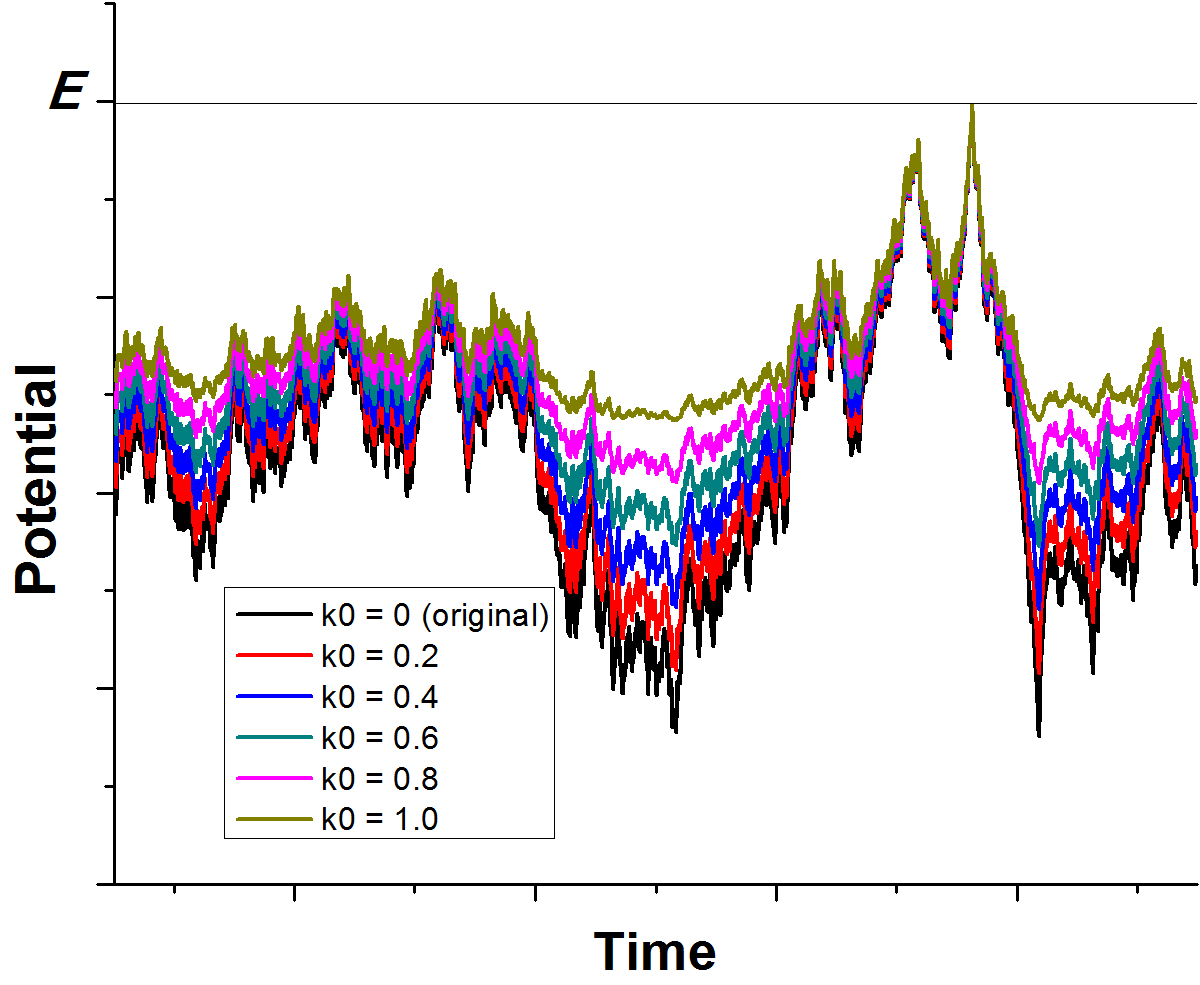
\includegraphics[width=7cm]{figures/GaMD-scheme.jpg}
  \caption{Schematic illustration of GaMD. When the threshold energy $E$ is set to the maximum potential ($iE=1$ mode), the system's potential energy surface is smoothened by adding a harmonic boost potential that follows a Gaussian distribution. The coefficient $k_0$, which falls in the range of $0 - 1.0$, determines the magnitude of the applied boost potential.}
  \label{fig:gamd_schematic}
\end{figure}

Consider a system with $N$ atoms at positions ${\bf r} = \big\{{\bf r}_1,\cdots,{\bf r}_N \}$. 
When the system's potential energy $V({\bf r})$ is lower than a threshold energy $E$, the following boost potential is added:
\begin{equation}
V^*({\bf r})= V({\bf r}) + \Delta V({\bf r}),
\end{equation}
where $\Delta V({\bf r})$ is the boost potential, 
\begin{equation} 
\Delta V({\bf r})= \left \{
\begin{array}{l l}
\frac{1}{2} k \left( E - V({\bf r}) \right)^2,  & \qquad V({\bf r})<E \\
0,   & \qquad V({\bf r})\geq E. \\  
\end{array} \right. 
\end{equation}
where $k$ is the harmonic force constant.

As explained in reference~\cite{MIAO2015mc}, the two adjustable parameters $E$ and $k$ are automatically determined by the following three criteria. 
First, $\Delta V$ should not change the relative order of the biased potential values, i.e., for any two arbitrary potential values $V_1 (\bf r)$ and $V_2 (\bf r)$ found on the original energy surface, if $V_1 ({\bf r}) < V_2 ({\bf r})$, 
then one should have $ V_1^* ({\bf r}) < V_2^* ({\bf r})$.
Second, the difference between potential energy values on the smoothened energy surface should be smaller than that of the original, 
i.e., if $V_1 ({\bf r}) < V_2 ({\bf r})$,  then one should have $ V_2^* ({\bf r}) - V_1^* ({\bf r}) < V_2 ({\bf r}) - V_1 ({\bf r})$.
By combining the above two criteria and plugging in the formula of $V^* ({\bf r})$ and $\Delta V$, one obtains
\begin{equation}
V_\text{max} \leq E \leq V_\text{min} + \frac{1}{k}
\label{eqn:limit}
\end{equation}
where $V_\text{min}$ and $V_\text{max}$ are the system's minimum and maximum potential energies. To ensure that Eqn.\,(\ref{eqn:limit}) is valid, $k$ needs 
to satisfy: $k \leq \frac{1}{ V_\text{max} - V_\text{min} }$. 
Define $k \equiv k_0 \cdot \frac{1}{V_\text{max} - V_\text{min}}$, then $0 < k_0 \leq 1$.
Third, the standard deviation of $\Delta V$ needs to be small enough (i.e., narrow distribution) to ensure accurate reweighting using cumulant expansion to the second order: 
$\sigma_{\Delta V} = k \left( E - V_\text{avg} \right) \sigma_V \leq \sigma_0$, 
where $V_\text{avg}$ and $\sigma_V$ are the average and standard deviation of the system's potential energies, 
$\sigma_{\Delta V}$ is the standard deviation of $\Delta V$, while $\sigma_0$ is a user-specified upper limit (e.g., $10 k_B T$) in order to achieve accurate reweighting.

{\bf iE = 1 mode:} When $E$ is set to $E = V_\text{max}$ according to Eqn.\,(\ref{eqn:limit}), 
$k_0$ is calculated as:
\begin{equation}
k_0 = \min(1.0, k'_0) = \min \left( 1.0, \frac{\sigma_0}{\sigma_V} \cdot
\frac{V_\text{max} - V_\text{min}}{V_\text{max} - V_\text{avg}} \right)
\label{eqn:mode1}
\end{equation}

{\bf iE = 2 mode:} Alternatively, when $E$ is set to $E = V_\text{min} + \frac{1}{k}$, 
$k_0$ is calculated as:
\begin{equation}
k_0 = k''_0 \equiv \left( 1 - \frac{\sigma_0}{\sigma_V} \cdot 
\frac{V_\text{max} - V_\text{min}}{V_\text{avg} - V_\text{min}} \right)
\label{eqn:mode2}
\end{equation}
If $k''_0$ obtained from the above equation is smaller than 0 or greater than 1, then $k_0$ will be calculated using Eqn.\,(\ref{eqn:mode1}).

For more details on GaMD and the corresponding reweighting using cumulant expansion, see reference~\cite{MIAO2015mc}\cite{PANG2017mc}. 

\subsubsection{NAMD parameters}

Same as aMD, three modes are available for applying boost potential in GaMD: 
(1) boosting the dihedral energy only, 
(2) boosting the total potential energy, and 
(3) boosting both the dihedral and total potential energy (i.e., ``dual-boost").

Some parameters from aMD, including: {\tt accelMD}, {\tt accelMDdihe}, {\tt accelMDdual}, {\tt accelMDFirstStep}, {\tt accelMDLastStep} and {\tt accelMDOutFreq} are shared by GaMD (see Section \ref{section:accelmd} for details).
The following is a list of input parameters unique to a GaMD run:

\begin{itemize}

\item
\NAMDCONFWDEF{accelMDG}{Is Gaussian accelerated MD on?}
{{\tt on} or {\tt off}}{{\tt off}}
{Specifies whether Gaussian accelerated MD (GaMD) is on. Only available when {\tt accelMD} is on. 
}

\item
\NAMDCONFWDEF{accelMDGiE}{Flag to set the threshold energy for adding boost potential}
{1 or 2}{1}
{Specifies how the threshold energy $E$ is set in GaMD. A value of 1 indicates that the threshold energy $E$ is set to its lower bound $E = V_\text{max}$. A value of 2 indicates that the threshold energy is set to its upper bound $E = V_\text{min} + (V_\text{max} - V_\text{min}) / k_0.$
}

\item
\NAMDCONFWDEF{accelMDGcMDPrepSteps}{Number of preparatory cMD steps}
{Zero or Positive integer}{200,000}
{The number of preparatory conventional MD (cMD) steps in GaMD. This value should be smaller than {\tt accelMDGcMDSteps} (see below). Potential energies are not collected for calculating the values of $V_\text{max}$, $V_\text{min}$, $V_\text{avg}$, $\sigma_V$ during the first {\tt accelMDGcMDPrepSteps}. 
}

\item
\NAMDCONFWDEF{accelMDGcMDSteps}{Number of total cMD steps}
{Zero or Positive integer}{1,000,000}
{The number of total cMD steps in GaMD. With ${\tt accelMDGcMDPrepSteps} < t < {\tt accelMDGcMDSteps}$, $V_\text{max}$, $V_\text{min}$, $V_\text{avg}$, $\sigma_V$ are collected and at $t = {\tt accelMDGcMDSteps}$, $E$ and $k_0$ are computed.
}

\item
\NAMDCONFWDEF{accelMDGEquiPrepSteps}{Number of preparatory equilibration steps in GaMD}
{Zero or Positive integer}{200,000}
{The number of preparatory equilibration steps in GaMD. This value should be smaller than {\tt accelMDGEquiSteps} (see below). With ${\tt accelMDGcMDSteps} < t < {\tt accelMDGEquiPrepSteps}+{\tt accelMDGcMDSteps}$, GaMD boost potential is applied according to $E$ and $k_0$ obtained at $t={\tt accelMDGcMDSteps}$. 
}

\item
\NAMDCONFWDEF{accelMDGEquiSteps}{Number of total equilibration steps in GaMD}
{Zero or Positive integer}{1,000,000}
{The number of total equilibration steps in GaMD. With ${\tt accelMDGEquiPrepSteps}+{\tt accelMDGcMDSteps} < t < {\tt accelMDGEquiSteps} +{\tt accelMDGcMDSteps}$, GaMD boost potential is applied, and $E$ and $k_0$ are updated every step.
}

\item
\NAMDCONFWDEF{accelMDGStatWindow}{Number of steps to calculate average and standard deviation in GaMD}
{Integer}{-1}
{The number of simulation steps used to calculate the average and standard deviation of potential energies, as well as the frequency of recalculating the boost potential during equilibration steps. When it is set to a negative number, all the steps throughout the cMD and equilibration stage (except the preparatory steps) will be used to calculate the average and standard deviation without resetting, and the boost potential will be updated every step during equilibration steps. When used, it is recommended to be set to about 4 times the total number of atoms in the system. Note that {\tt accelMDGcMDPrepSteps}, {\tt accelMDGcMDSteps}, {\tt accelMDGEquiPrepSteps} and {\tt accelMDGEquiSteps} need to be multiples of {\tt accelMDGStatWindow}.
}

\item
\NAMDCONFWDEF{accelMDGSigma0P}{Upper limit of the standard deviation of the total boost potential in GaMD}
{Positive real number}{6.0 (kcal/mol)}
{Specifies the upper limit of the standard deviation of the total boost potential. This option is only available when {\tt accelMDdihe} is off or when {\tt accelMDdual} is on.
}

\item
\NAMDCONFWDEF{accelMDGSigma0D}{Upper limit of the standard deviation of the dihedral boost potential in GaMD}
{Positive real number}{6.0 (kcal/mol)}
{Specifies the upper limit of the standard deviation of the dihedral boost potential. This option is only available when {\tt accelMDdihe} or {\tt accelMDdual} is on.
}

\item
\NAMDCONFWDEF{accelMDGRestart}{Flag to restart GaMD simulation}
{{\tt on} or {\tt off}}{{\tt off}}
{Specifies whether the current GaMD simulation is the continuation of a previous run. If this option is turned on, the GaMD restart file specified by {\tt accelMDGRestartFile} (see below) will be read. 
}

\item
\NAMDCONF{accelMDGRestartFile}{Name of GaMD restart file}
{UNIX filename}
{A GaMD restart file that stores the current number of steps, maximum, minimum, average and standard deviation of the dihedral and/or total potential energies (depending on the {\tt accelMDdihe} and {\tt accelMDdual} parameters). This file is saved automatically every {\tt restartfreq} steps. If {\tt accelMDGRestart} is turned on, this file will be read and the simulation will restart from the point where the file was written.
}

\end{itemize}


\subsection{Solute Scaling and REST2}
\label{section:rest2}

Solute scaling improves sampling efficiency
by scaling the intramolecular potential energy of a protein
to lower barriers separating different confirmations~\cite{WANG2011E}.
The potential is scaled based on a parameter $\beta$,
\begin{equation}
U^{\text{SS}}(\vec{r}) =
\beta U_{\text{pp}}(\vec{r}) +
\sqrt{\beta} U_{\text{pw}}(\vec{r}) +
U_{\text{ww}}(\vec{r}),
\end{equation}
with $U_{\text{pp}}$ denoting protein--protein interactions,
$U_{\text{pw}}$ denoting protein--water interactions,
and $U_{\text{ww}}$ denoting water--water interactions,
effectively ``heating'' the protein's interatomic interactions
whenever $\beta < 1$.
The NAMD implementation is made efficient by rescaling
the force field parameters for the affected atoms~\cite{JO2015}.
In particular, this parameter scaling approach makes the calculation
compatible with existing CUDA force kernels.

The NAMD implementation provides additional flexibility to
solute scaling by allowing different scaling factors for electrostatics,
van der Waals, and bonded interactions, as described in the
following section.
Solute scaling can be combined with replica exchange
to produce a powerful sampling enhancement method
that is highly transferable and provides higher efficiency
than traditional temperature exchange methods.
In the literature, this replica exchange solute scaling method
is known as REST2, due to its improvement of the earlier
REST (replica exchange solute tempering) method
that directly scaled the temperature of the solute.
Sample files are available in directory {\tt lib/replica/REST2},
with script file {\tt lib/replica/REST2/rest2\_remd.namd}
demonstrating use of solute scaling with multiple replicas.

\subsubsection{NAMD parameters}

The following parameters are used to control solute scaling:

\begin{itemize}

\item
\NAMDCONFWDEF{soluteScaling}{%
Is replica exchange solute tempering enabled?
}{%
{\tt on} or {\tt off}}{{\tt off}
}{%
Specifies whether or not REST2 is enabled.
If set on, then {\tt soluteScaling} must also be set.
}

\item
\NAMDCONFWDEF{soluteScalingFactor}{%
Solute scaling factor
}{%
non-negative
}{%
1.0
}{%
This option sets the scaling factor $\beta$, and is typically set lower
than 1 to reduce potential energy barriers for the solute.
In a replica-exchange run, this option and the related options
{\tt soluteScalingFactorCharge} and {\tt soluteScalingFactorVdw} serve also as
Tcl scripting commands to update the corresponding parameters during a
simulation.
{\em After using} {\tt reinitatoms}{\em it is highly recommended that these
  commands are repeated even if the corresponding parameters are not being
  updated, to preserve their intended value.}
}

\item
\NAMDCONFWDEF{soluteScalingFactorCharge}{%
Solute scaling factor for electrostatics
}{%
non-negative}{{\tt soluteScalingFactor}
}{%
Scaling factor applied to just the electrostatics interactions.
If not specified, this is set to {\tt soluteScalingFactor}.
}

\item
\NAMDCONFWDEF{soluteScalingFactorVdw}{%
Solute scaling factor for van der Waals
}{%
non-negative}{{\tt soluteScalingFactor}
}{%
Scaling factor applied to just the van der Waals interactions.
If not specified, this is set to {\tt soluteScalingFactor}.
}

\item
\NAMDCONFWDEF{soluteScalingFile}{%
PDB file with scaling flags
}{%
UNIX filename}{{\tt coordinates}
}{%
PDB file used to flag solute atoms for scaling.
If undefined, this defaults to the coordinate PDB file.
}

\item
\NAMDCONFWDEF{soluteScalingCol}{%
Column of PDB file
}{%
{\tt X}, {\tt Y}, {\tt Z}, {\tt O}, or {\tt B}}{{\tt O}
}{%
Column of the PDB file used to flag solute atoms for scaling.
If undefined, this defaults to the {\tt O} (occupancy) column.
A value of 1.0 marks the atom for scaling.
}

\item
\NAMDCONFWDEF{soluteScalingAll}{%
Apply scaling also to bond and angle interactions?
}{%
{\tt on} or {\tt off}}{{\tt off}
}{%
If set on, {\tt scalingFactor} is applied also to bond and angle interactions.
Otherwise, {\tt scalingFactor} is applied only to dihedral, improper,
and crossterm interactions.
}

\end{itemize}


\subsection{Adaptive Tempering}
\label{section:adapttemp}
Adaptive tempering is akin to a single-copy replica exchange method for dynamically updating the simulation temperature. The temperature $T$ is a new random variable in the range $[Tmin,Tmax]$ that is governed by the equation $dE/dT = E-E(T)-1/T+sqrt(2)T\xi$, where $\xi$ is Gaussian white noise. The effect is that when the potential energy for a given structure is lower than the (so far calculated) average energy, the temperature is lowered. Conversely when the current energy is higher than the average energy, the temperature is raised. The effect is faster conformational sampling to find minimum energy structures. The method is implemented exactly as described by Zhang and Ma in J. Chem. Phys. 132, 244101 (2010) (using Equation 18 of their paper to calculate the average energy at a given temperature from the histogram of energies). 

The dynamic temperature is realized either by changing the temperature of the Langevin thermostat or by velocity rescaling. 

\subsubsection{NAMD parameters}

The following parameters are used to adaptive tempering:

\begin{itemize}

\item
\NAMDCONFWDEF{adaptTempMD}{Is adaptive tempering active?}{{\tt on} or {\tt
off}}{{\tt off}}
{Specifies whether or not adaptive tempering is used. If set to on then the following parameters are required to be set: either all of ({\tt adaptTempTmin}, {\tt adaptTempTmax}, {\tt adaptTempBins}, {\tt adaptTempDt}) or {\tt adaptTempInFile} (but not both).
}

\item
\NAMDCONFWDEF{adaptTempFreq}{steps between temperature updates}
{Positive integers}{10}
{The number of steps between temperature updates. Note that the potential energy at the current is calculated and added to the temperature-energy histogram at every step.
}

\item
\NAMDCONF{adaptTempTmin}{minimum temperature (K)}
{Positive real number} 
{Sets the minimum temperature to be used in the simulation.
}

\item
\NAMDCONF{adaptTempTmax}{maximum temperature (K)}
{Positive real number}
{Sets the maximum temperature to be used in the simulation.
}

\item
\NAMDCONFWDEF{adaptTempBins}{number of temperature bins}
{Positive integer}{1000}
{Sets the number of bins to subdivide the temperature range. Each bin stores the average energy for the given temperature 
}

\item
\NAMDCONFWDEF{adaptTempDt}{stepsize for temperature updates}{Positive real numbers}{$10^{-4}$}
{Integration timestep for temperature updates. This is unrelated to the simulation timestep and only scales the size of the step taken in temperature space every {\tt adaptTempFreq} steps.
}

\item
\NAMDCONF{adaptTempInFile}{adaptive tempering input filename}
{UNIX filename}
{The input file containing restart information for adaptive tempering (written out by {\tt adaptTempRestartFile}).
}

\item
\NAMDCONF{adaptTempRestartFile}{adaptive tempering restart filename}
{UNIX filename}
{The file to write out restart information for adaptive tempering.
}

\item
\NAMDCONF{adaptTempRestartFreq}{steps between writing restart file}
{Positive integer}
{Frequency of writing restart file.
}

\item
\NAMDCONFWDEF{adaptTempLangevin}{send temperature updates to langevin thermostat?}
{{\tt on} or {\tt off}}{{\tt on}}
{Setting this to on will cause the langevin thermostat to use the updated temperatures from adaptive tempering. Note that either one of adaptTempLangevin or adaptTempRescaling have to be on.
}

\item
\NAMDCONFWDEF{adaptTempRescaling}{send temperature to velocity rescaling thermostat?}
{{\tt on} or {\tt off}}{{\tt on}}
{Setting this to on will cause the veloctiy rescaling thermostat to use the updated temperatures from adaptive tempering.  Note that either one of adaptTempLangevin or adaptTempRescaling have to be on.
}

\item
\NAMDCONFWDEF{adaptTempOutFreq}{steps between printing adaptive tempering output}
{Positive integers}{10}
{The number of timesteps between printing adaptive tempering output to the log file.
}

\item
\NAMDCONFWDEF{adaptTempFirstStep}{step to start adaptive tempering}
{Non-negative integers}{0}
{The first timestep from which adaptive tempering will be run.}

\item
\NAMDCONF{adaptTempLastStep}{step to stop adaptive tempering}
{Positive integers}
{The last timestep to apply adaptive tempering.}

\item
\NAMDCONFWDEF{adaptTempCgamma}{dynamic bin averaging constant}
{Non-negative real number}{0.1}
{The calculation of the mean energy for a given bin is weighted by a factor of 1 - Cgamma / samples to damp out old statistics. Setting Cgamma to zero restores the use of a standard arithmetic mean to calculate the mean energy for each bin.}

\item
\NAMDCONFWDEF{adaptTempRandom}{assign random temperature if we step out of range?}
{{\tt on} or {\tt off}}{{\tt off}}
{If set to on and the temperature steps out of [{\tt adaptTempTmin}, {\tt adaptTempTmax}], a random temperature in that range is assigned. Otherwise the previous temperature is kept.
}

%\item
%\NAMDCONFWDEF{adaptTempDebug}{print debug output?}
%{{\tt on} or {\tt off}}{{\tt off}}
%{Print adaptive tempering debug output.
%}

\end{itemize}


\subsection{Locally enhanced sampling}
\label{section:les}

Locally enhanced sampling (LES)~\cite{ROIT91,SIMM98,SIMM00} increases
sampling and transition rates for a portion of a molecule by the use of
multiple non-interacting copies of the enhanced atoms.  These enhanced
atoms experience an interaction (electrostatics, van der Waals, and
covalent) potential that is divided by the number of copies present.
In this way the enhanced atoms can occupy the same space, while the
multiple instances and reduces barriers increase transition rates.

\subsubsection{Structure generation}

To use LES, the structure and coordinate input files must be modified to
contain multiple copies of the enhanced atoms.  \PSFGEN\ provides the
{\tt multiply} command for this purpose.  \NAMD\ supports a maximum of 255
copies, which should be sufficient.  

Begin by generating the complete molecular structure and guessing
coordinates as described in Sec.~\ref{section:psfgen}.  As the last
operation in your script, prior to writing the psf and pdb files, add
the {\tt multiply} command, specifying the number of copies desired and
listing segments, residues, or atoms to be multiplied.  For example,
\verb#multiply 4 BPTI:56 BPTI:57# will create four copies of the last
two residues of segment BPTI.  You must include all atoms to be
enhanced in a single {\tt multiply} command in order for the bonded
terms in the psf file to be duplicated correctly.  Calling {\tt multiply}
on connected sets of atoms multiple times will produce unpredictable
results, as may running other commands after {\tt multiply}.

The enhanced atoms are duplicated exactly in the structure---they have
the same segment, residue, and atom names.  They are distinguished only
by the value of the B (beta) column in the pdb file, which is 0 for
normal atoms and varies from 1 to the number of copies created for
enhanced atoms.  The enhanced atoms may be easily observed in VMD with
the atom selection \verb#beta != 0#.

\subsubsection{Simulation}

In practice, LES is a simple method used to increase sampling;
no special output is generated.
The following parameters are used to enable LES:

\begin{itemize}

\item
\NAMDCONFWDEF{les}{is locally enhanced sampling active?}{{\tt on} or {\tt
off}}{{\tt off}}
{Specifies whether or not LES is active.}

\NAMDCONF{lesFactor}{number of LES images to use}
{positive integer equal to the number of images present}
{This should be equal to the factor used in {\tt multiply}
 when creating the structure.  The interaction potentials for images is
 divided by {\tt lesFactor}.  
}

\item
\NAMDCONFWDEF{lesReduceTemp}{reduce enhanced atom temperature?}{{\tt on} or {\tt
off}}{{\tt off}}
{Enhanced atoms experience interaction potentials divided by {\tt lesFactor}.
This allows them to enter regions that would not normally be thermally
accessible.  If this is not desired, then the temperature of these atoms
may be reduced to correspond with the reduced potential.  This option
affects velocity initialization, reinititialization, reassignment, and
the target temperature for langevin dynamics.  Langevin dynamics is
recommended with this option, since in a constant energy simulation energy
will flow into the enhanced degrees of freedom until they reach thermal
equilibrium with the rest of the system.  The reduced temperature atoms
will have reduced velocities as well, unless {\tt lesReduceMass} is also
enabled.}

\item
\NAMDCONFWDEF{lesReduceMass}{reduce enhanced atom mass?}{{\tt on} or {\tt off}}{{\tt off}}
{Used with {\tt lesReduceTemp} to restore velocity distribution to
enhanced atoms.  If used alone, enhanced atoms would move faster than
normal atoms, and hence a smaller timestep would be required.}

\item
\NAMDCONFWDEF{lesFile}{PDB file containing LES flags}{UNIX filename} {{\tt coordinates}}
{PDB file to specify the LES image number of each atom.
If this parameter is not specified, then 
the PDB file containing initial coordinates specified by 
{\tt coordinates} is used.}

\item
\NAMDCONFWDEF{lesCol}{column of PDB file containing LES flags}{{\tt X}, {\tt Y}, {\tt Z}, {\tt O}, or {\tt B}}{{\tt B}}
{Column of the PDB file to specify the LES image number of each atom.
This parameter may specify any of the floating point fields of the PDB file, 
either X, Y, Z, occupancy, or beta-coupling (temperature-coupling).  
A value of 0 in this column indicates that the atom is not enhanced.
Any other value should be a positive integer less than {\tt lesFactor}.}

\end{itemize}


\subsection{Replica exchange simulations}

\index{replica exchange}
The {\tt lib/replica/}
directory contains Tcl scripts that implement replica exchange
both for parallel tempering (temperature exchange) and
umbrella sampling (exchanging collective variable biases).
This replaces the old Tcl server and socket connections driving a
separate NAMD process for every replica used in the simulation.

{\bf A NAMD build based on Charm++ 6.5.0 or later using one of the
``LRTS'' (low-level runtime system) machine layers is required!}
Current LRTS machine layers include mpi, netlrts, verbs (for InfiniBand),
gemini\_gni-crayxe, gni-crayxc, and pamilrts-bluegeneq.

Only temperature-exchange simulations are described below.
To employ replicas for umbrella sampling you will need to understand
this material, collective variable-based calculations (Sec.\ \ref{section:colvars}),
and basic Tcl programming to adapt the examples in {\tt lib/replica/umbrella/}
and {\tt lib/replica/umbrella2d/} until further
documentation and a tutorial are available.

This implementation is designed to be modified to implement
exchanges of parameters other than temperature or via other temperature
exchange methods.  The scripts should provide a good starting point for
any simulation method requiring a number of loosely interacting systems.

Replica exchanges and energies are recorded in the .history files
written in the output directories.  These can be viewed with, e.g.,
``{\tt xmgrace output/*/*.history}'' and processed via awk or other tools.
There is also a script to load the output into VMD and color each
frame according to replica index.  An example simulation folds
a 66-atom model of a deca-alanine helix in about 10\,ns.

{\tt replica.namd}
is the master script for replica temperature-exchange simulations.  To run:
\begin{verbatim}
          cd example
          mkdir output
          (cd output; mkdir 0 1 2 3 4 5 6 7)
          mpirun namd3 +replicas 8 job0.conf +stdout output/%d/job0.%d.log
          mpirun namd3 +replicas 8 job1.conf +stdout output/%d/job1.%d.log
\end{verbatim}

The number of MPI ranks must be a multiple of the number of replicas
(+replicas).  Be sure to increment jobX for +stdout option on command line.

{\tt show\_replicas.vmd} is a script for loading replicas into VMD;
first source the replica exchange conf file and then this script, then
repeat for each restart conf file or for example just do
``{\tt vmd -e load\_all.vmd}''.
This script will likely destroy anything else you are doing in VMD at the
time, so it is best to start with a fresh VMD.
{\tt clone\_reps.vmd} provides the {\tt clone\_reps} commmand to copy graphical
representation from the top molecule to all other molecules.

{\tt sortreplicas}, found in the namd3 binary directory, is a program to un-shuffle
replica trajectories to place same-temperature frames in the same file.
Usage:
\begin{verbatim}
  sortreplicas <job_output_root> <num_replicas> <runs_per_frame> [final_step]
\end{verbatim}
where job\_output\_root is the job specific output base path, including
\%s or \%d for separate directories as in output/\%s/fold\_alanin.job1
This will be extended with .\%d.dcd .\%d.history for input files and
.\%d.sort.dcd .\%d.sort.history for output files.  The optional final\_step
parameter will truncate all output files after the specified step,
which is useful in dealing with restarts from runs that did not complete.
Colvars trajectory files are similarly processed if they are found.

A replica exchange config file should define the following Tcl variables:
\begin{itemize}
\item {\tt num\_replicas}, the number of replica simulations to use,
\item {\tt min\_temp}, the lowest replica target temperature,
\item {\tt max\_temp}, the highest replica target temperature,
\item {\tt steps\_per\_run}, the number of steps between exchange attempts,
\item {\tt num\_runs}, the number of runs before stopping
(should be divisible by {\tt runs\_per\_frame} $\times$ {\tt frames\_per\_restart}).
\item {\tt runs\_per\_frame}, the number of runs between trajectory outputs,
\item {\tt frames\_per\_restart}, the number of frames between restart outputs,

\item {\tt namd\_config\_file}, the NAMD config file containing all parameters,
needed for the simulation except {\tt seed}, {\tt langevin}, 
{\tt langevinTemp}, {\tt outputEnergies},
{\tt outputname}, {\tt dcdFreq},
{\tt temperature}, {\tt bincoordinates}, {\tt binvelocities},
or {\tt extendedSystem}, which are provided by {\tt replica.namd},

\item {\tt output\_root}, the directory/fileroot for output files,
optionally including a ``\%s'' that is replaced with the replica index
to use multiple output directories,

\item {\tt psf\_file}, the psf file for {\tt show\_replicas.vmd}, 
\item {\tt initial\_pdb\_file}, the initial coordinate pdb file for {\tt show\_replicas.vmd},
\item {\tt fit\_pdb\_file}, the coodinates that frames are fit to by {\tt show\_replicas.vmd} (e.g., a folded structure),
\end{itemize}

The {\tt lib/replica/example/} directory contains
all files needed to fold a 66-atom model of a deca-alanine helix:
\begin{itemize}
\item {\tt alanin\_base.namd}, basic config options for NAMD,
\item {\tt alanin.params}, parameters,
\item {\tt alanin.psf}, structure,
\item {\tt unfolded.pdb}, initial coordinates,
\item {\tt alanin.pdb}, folded structure for fitting in {\tt show\_replicas.vmd},
\item {\tt fold\_alanin.conf}, config file for {\tt replica\_exchange.tcl} script,
\item {\tt job0.conf}, config file to start alanin folding for 10\,ns,
\item {\tt job1.conf}, config file to continue alanin folding another 10\,ns, and
\item {\tt load\_all.vmd}, load all output into VMD and color by replica index.
\end{itemize}

The {\tt fold\_alanin.conf} config file contains the following settings:
\begin{verbatim}
set num_replicas 8
set min_temp 300
set max_temp 600
set steps_per_run 1000
set num_runs 10000
# num_runs should be divisible by runs_per_frame * frames_per_restart
set runs_per_frame 10
set frames_per_restart 10
set namd_config_file "alanin_base.namd"
set output_root "output/%s/fold_alanin" ; # directories must exist

# the following used only by show_replicas.vmd
set psf_file "alanin.psf"
set initial_pdb_file "unfolded.pdb"
set fit_pdb_file "alanin.pdb"
\end{verbatim}

\subsection{Random acceleration molecular dynamics simulations}

The ``lib/ramd" directory stores the tcl scripts and the example files for the implementation of the Random Acceleration Molecular Dynamics (RAMD) simulation method in NAMD. 
The RAMD method can be used to carry out molecular dynamics (MD) simulations with an additional randomly oriented acceleration applied to the center of mass of one group of atoms (referred to below as ``ligand") in the system. 
It can, for example, be used to identify egress routes for a ligand from a buried protein binding site. 
Since its original implementation in the ARGOS \mycite{L{\"u}demann \ETAL, 2000}{ludemann2000substrates,winn2002comparison} program, the method has been implemented in AMBER 8 \mycite{Schleinkofer \ETAL, 2005}{schleinkofer2005mammalian}, and CHARMM \mycite{Carlsson \ETAL, 2006}{carlsson2006unbinding}. 
The first implementation of RAMD in NAMD using a tcl script (available as supplementary material in \mycite{Vashisth \ETAL, 2008}{vashisth2008ligand}) provided only limited functionality compared to the AMBER 8 implementation and was followed with an implementation of RAMD and RAMD--MD in NAMD \mycite{}{cojocaru2012multiple,biedermannova2012single}. Recently the RAMD method was improved in speed by using NAMD vector implementations and streamlining the code. The current implementation is now focused on the RAMD simulation and was used in the $\tau$RAMD procedure for the estimation of relative drug-target residence times \mycite{Kokh \ETAL, 2018}{kokh2018estimation}.

Additional information is found in the README file in the ``lib/ramd" directory. 
The user is encouraged to carefully read this information before starting production runs.

The two required scripts are stored in ``lib/ramd/scripts": (i) ramd--5.tcl defines the simulation parameters and passes them from the NAMD configuration file to the main script, (ii) ``ramd--5\_script.tcl" adds the randomly oriented force and performs all related computations.

Two examples for running RAMD are included in the directory ``lib/ramd/example/". The examples can be started using the RAMD-force.sh shell scripts.

The specific RAMD simulation parameters to be provided in the NAMD configuration file (listed below) should be preceded by the keyword ``ramd". 
The default values for these parameters are only given as guidance. 
They may not to be suitable for other systems. 

Mandatory parameter settings:\\
\begin{itemize}
\item
\NAMDCONF{ramd lastProtAtom} {Last index of protein atom} {{\tt positive integer}} { Specifies the index of the last protein atom. } 

\item
\NAMDCONF{ramd firstRamdAtom}{ First index of ligand atom } {{\tt positive integer}} {Specifies the index of the first ligand atom.}

\item
\NAMDCONF{ramd lastRamdAtom}{ Last index of ligand atom } {{\tt positive integer}} {Specifies the index of the last ligand atom. }

\item
\NAMDCONF{ramd ramdfilename}{Name of ramd output file}{{\tt Valid file name}}{Specified the name of the file where the ramd logs are written.}
\end{itemize}

Optional parameter settings with a default. Depending on your simulation system, you might want to change these settings:\\
\begin{itemize}
\item
\NAMDCONFWDEF{ramd firstProtAtom} {First index of protein atom} {{\tt positive integer}} {{\tt 1}} { Specifies the index of the first protein atom.}
 
\item
\NAMDCONFWDEF{ramd ramdSteps} { Set number of steps in RAMD block} {{\tt positive integer}} {{\tt 50}} {Specifies the number of steps in 1 RAMD block; the simulations are evaluated every `ramdSteps' steps.} 

\item
\NAMDCONFWDEF{ramd forceRAMD} {Set acceleration force} {{\tt positive decimal}} {{\tt 16.0}} {Specifies the force to be applied. Replaces the acceleration (accel) specified in previous releases. Defaults to 16 kcal/mol/Angstrom}

\item
\NAMDCONFWDEF{ramd rMinRamd} {Set threshold for distance travelled RAMD} {{\tt positive decimal}} {{\tt 0.01}} {Specifies a threshold value for the distance in Angstroms travelled by the ligand in 1 RAMD block. In RAMD simulations the direction of the acceleration is changed if the ligand has travelled less than `rMinRamd' \AA\ in the evaluated block. 
%(In combined RAMD-MD simulations, a switch from a RAMD block to a standard MD block is applied if the ligand travelled more than `rMinRamd' \AA in the evaluated block.)
}

\item
\NAMDCONFWDEF{ramd forceOutFreq}{Set frequency of RAMD forces output} {{\tt positive integer}, Must be divisor of {\tt ramdSteps}} {{\tt 10}} { Every `forceOutFreq' steps, detailed output of forces will be written.} 

\item
\NAMDCONFWDEF{ramd maxDist} {Set center of mass separation} {{\tt positive decimal}} {{\tt 50}} { Specifies the distance in Angstroms between the the centers of mass of the ligand and the protein when the simulation is stopped.}
 

\item
\NAMDCONFWDEF{ramd ramdSeed}{Set RAMD seed} {{\tt positive integer}} {{\tt 14253}} {Specifies seed for the random number generator for generation of RAMD force directions. Change this parameter if you wish to run different trajectories with identical parameters.}

\item
\NAMDCONFWDEF{ramd debugLevel}{ Set debug level of RAMD} {\tt integer value } {0} { Activates verbose output if set to an integer greater than 0. Should be used only for testing purposes because the very dense output is full of information only relevant for debugging.}

\item
\NAMDCONFWDEF{ramd namdVersion}{ Set the NAMD version}{\tt float value } {2.13} { After NAMD version 2.10 a call to {\em enabletotalforces} is done to enable tcl processing in NAMD}

\end{itemize}

Note: 
In the current RAMD implementation, combined RAMD-MD simulations, where RAMD blocks alternate with standard MD blocks are not available. In case you are are interested in this feature, please contact the RAMD developers at mcmsoft@h-its.org

Scripts for using RAMD in the $\tau$RAMD procedure for computing residence times are available at: \url{https://www.h-its.org/downloads/ramd/}.
 

